%%%%%%%%%%%%%%%%%%% vorlage.tex %%%%%%%%%%%%%%%%%%%%%%%%%%%%%
%
% LaTeX-Vorlage zur Erstellung von Projekt-Dokumentationen
% im Fachbereich Informatik der Hochschule Trier
%
% Basis: Vorlage svmono des Springer Verlags
%
%%%%%%%%%%%%%%%%%%%%%%%%%%%%%%%%%%%%%%%%%%%%%%%%%%%%%%%%%%%%%

\documentclass[envcountsame,envcountchap, deutsch]{i-studis}

\usepackage{makeidx}         	% Index
\usepackage{multicol}        	% Zweispaltiger Index
%\usepackage[bottom]{footmisc}	% Erzeugung von Fu�noten

%%-----------------------------------------------------
%\newif\ifpdf
%\ifx\pdfoutput\undefined
%\pdffalse
%\else
%\pdfoutput=1
%\pdftrue
%\fi
%%--------------------------------------------------------
%\ifpdf
\usepackage[pdftex]{graphicx}
\usepackage[pdftex,plainpages=false]{hyperref}
%\else
%\usepackage{graphicx}
%\usepackage[plainpages=false]{hyperref}
%\fi

%%-----------------------------------------------------
\usepackage{color}				% Farbverwaltung
%\usepackage{ngerman} 			% Neue deutsche Rechtsschreibung
\usepackage[english, ngerman]{babel}
\usepackage[latin1]{inputenc} 	% Erm�glicht Umlaute-Darstellung
%\usepackage[utf8]{inputenc}  	% Erm�glicht Umlaute-Darstellung unter Linux (je nach verwendetem Format)

%-----------------------------------------------------
\usepackage{listings} 			% Code-Darstellung
\lstset
{
	basicstyle=\scriptsize, 	% print whole listing small
	keywordstyle=\color{blue}\bfseries,
								% underlined bold black keywords
	identifierstyle=, 			% nothing happens
	commentstyle=\color{red}, 	% white comments
	stringstyle=\ttfamily, 		% typewriter type for strings
	showstringspaces=false, 	% no special string spaces
	framexleftmargin=7mm, 
	tabsize=3,
	showtabs=false,
	frame=single, 
	rulesepcolor=\color{blue},
	numbers=left,
	linewidth=146mm,
	xleftmargin=8mm
}
\usepackage{textcomp} 			% Celsius-Darstellung
\usepackage{amssymb,amsfonts,amstext,amsmath}	% Mathematische Symbole
\usepackage[german, ruled, vlined]{algorithm2e}
\usepackage[a4paper]{geometry} % Andere Formatierung
\usepackage{bibgerm}
\usepackage{array}
\hyphenation{Ele-men-tar-ob-jek-te  ab-ge-tas-tet Aus-wer-tung House-holder-Matrix Le-ast-Squa-res-Al-go-ri-th-men} 		% Weitere Silbentrennung bei Bedarf angeben
\setlength{\textheight}{1.1\textheight}
\pagestyle{myheadings} 			% Erzeugt selbstdefinierte Kopfzeile
\makeindex 						% Index-Erstellung


%--------------------------------------------------------------------------
\begin{document}
%------------------------- Titelblatt -------------------------------------
\title{Entwicklung eines 2D Plattformers}
\subtitle{Dokumentationn}
%---- Die Art der Dokumentation kann hier ausgew�hlt werden---------------
%\project{Bachelor-Projektarbeit}
\project{Medienprojekt}
%\project{Master-Projektstudium}
%\project{Master-Abschlussarbeit}
%\project{Seminar zur Vorlesung ...}
%\project{Hausarbeit zur Vorlesung ...}
%--------------------------------------------------------------------------
\supervisor{Prof. Dr. Christof Rezk-Salama} 		% Betreuer der Arbeit
\author{Fabio Gimmillaro, Daniel Schreiber, Tobias R"uhl und Joscha W"ulk} 							% Autor der Arbeit
\address{Trier,} 							% Im Zusammenhang mit dem Datum wird hinter dem Ort ein Komma angegeben
\submitdate{Abgabedatum} 				% Abgabedatum
%\begingroup
%  \renewcommand{\thepage}{title}
%  \mytitlepage
%  \newpage
%\endgroup
\begingroup
  \renewcommand{\thepage}{Titel}
  \mytitlepage
  \newpage
\endgroup
%--------------------------------------------------------------------------
\frontmatter 
%--------------------------------------------------------------------------
\tableofcontents 						% Inhaltsverzeichnis
%--------------------------------------------------------------------------
\mainmatter                        		% Hauptteil (ab hier arab. Seitenzahlen)
%--------------------------------------------------------------------------
% Die Kapitel werden in separaten .tex-Dateien abgelegt und hier eingebunden.
\chapter{Konzeptionierung}
\chapter{Die Kamera}
Die Kamera ist eine einfache Verfolgerkamera. Diese verfolgt die Spielerfigur, wenn sich dieser in X- oder Y-Richtung eine gewisse Entfernung entfernt, und f"ahrt je nach Entfernung langsamer oder schneller dem Spieler hinterher. Hierbei war es wichtig die Grenzen korrekt einzustellen, ab wann die Kamera dem Spieler verfolgen soll, um in allen Situationen den besten "Uberblick zu gew"ahren. So war es beispielsweise sinnvoll f"ur das Springen eine geringe Toleranz zu w"ahlen, sodass die Kamera schnell folgt. Andernfalls traten Probleme auf, einzusch"atzen wie in vertikalen Levels der Pfad zu w"ahlen ist.
Die ma"sgebliche Schleife f"ur die Kamera wird im LateUpdate von Unity aufgerufen, da dies geschehen soll, nachdem Bewegungen oder "Ahnliches im normalen Update durchgef"uhrt wurden.
Sie sieht folgenderma"sen aus:
\begin{lstlisting}[breaklines=true]
void LateUpdate()
{
	//Standartmaessig sind die gewuenschten Koordinaten, die unveraendert bleiben sollen.
	float targetX = transform.position.x+xOffset;
	float targetY = transform.position.y+yOffset;
	// Wenn der Spieler sich zu weit in X Richtung entfernt
	if (CheckXMargin ()) {
		//Soll der Zielpunkt dem Spieler hinterher interpolieren um eine glatte
		//Kamerafahrt zu ermoeglichen
		targetX = Mathf.Lerp(transform.position.x,player.position.x+xOffset, xSmooth * Time.deltaTime);
	}

	// Wenn der Spieler sich zu weit in Y Richtung entfernt
	if (CheckYMargin ()) {
		//Soll der Zielpunkt dem Spieler hinterher interpolieren um eine glatte
		//Kamerafahrt zu ermoeglichen
		targetY = Mathf.Lerp (transform.position.y,
		player.position.y+yOffset, ySmooth *
		Time.deltaTime);
	}
	
	//Fur Levelgrenzen wird der Zielwert auf Minimal- und Maximalwerte festgehalten
	targetX = Mathf.Clamp(targetX, minXAndY.x, maxXAndY.x);
	targetY = Mathf.Clamp(targetY, minXAndY.y, maxXAndY.y);
	//Setze die Kameraposition auf die errechnete Positon
	transform.position = new Vector3(targetX, targetY, transform.position.z);
}
\end{lstlisting}
\chapter{GameObject ``Player`` \& Komponenten}

Die Spielfigur, die der Anwender bedient stellte sich w"ahrend der Entwicklung als komplexestes GameObject heraus. In diesem Kapitel geben wir daher einen "Uberblick "uber die Realisierung mithilfe von Sprites sowie der verschiedenen anh"angenden und selbsterstellten Skripte

\begin{figure}
	\centering
	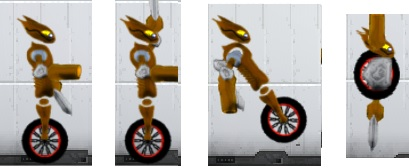
\includegraphics[height=5cm]{images/AnimationenZusammenschnitt.jpg}
	\caption{Zusammenschnitt der Player Sprites}
	\label{fig:playerSprites}
\end{figure}

\section{SpriteRenderer}

\section{AttributeComponent Skript}
Die AttributeComponent dient dazu die spielmechanischen Daten zu hinterlegen und zu verwalten. Sie kann sowohl dem Spieler als auch freundlich und feindlich Gesinnten NPCs angeh"angt werden. 

Nachfolgend werden die wichtigsten Daten vorgestellt:
\begin{lstlisting}[breaklines=true]
//Lebenspunkte, maximale Lebenspunkte, Ruestung und Schaden
public float health, maxHealth, armor, damage;
//Maximale Ausdauer, Ausdauer und regenerierte Ausdauer pro Sekunde
public float maxStamina, stamina, staminaPerSecond;
//Munition, Munitionskapazitaet und Reichweite
//Range = 0 -> Nahkampf / Range > 0 -> Fernkampf
public int ammo, ammoCap, range;
//Klon aktiv?
public bool cloneAlive = false;

//Cooldown fuer Plasmaschuss
static float cooldown1 = 1.0f;
//Laeuft cooldown fuer Plasmaschuss?
bool cooldown1Active = false;

//Cooldown fuer Klonfaehigkeit
static float cooldown2 = 10.0f;
//Time-to-live fuer Klon
static float ttl = 5.0f;
//Aktuelle Time-To-Live
float attl = ttl;
//Laeuft cooldown fuer Klon?
bool cooldown2Active = false;

//Referenz auf das Nahkampfsystem
MeleeSystem meleeSys;
\end{lstlisting}

Die Update-Funktion der AttributeComponent wird ausschlie"slich dazu benutzt, die Stamina "uber Zeit aufzuf"ullen w"ahrend die fixedUpdate-Funktion f"ur das l"oschen des Klones verantwortlich ist.
\begin{lstlisting}[breaklines=true]
void Update () {

/*Fuelle Ausdauer ueber Zeit wieder auf solange maximalStamina nicht erreicht ist und die
Spielfigur sich nicht bewegt*/
if (staminaPerSecond > 0.0f && stamina < maxStamina && !meleeSys.animationRunning)
{
//Stelle sicher, dass Stamina nicht kleiner als 0 oder groesser als maximalStamina gesetzt wird
stamina = Mathf.Clamp(stamina+staminaPerSecond * Time.deltaTime,0,maxStamina);
}   
}
void FixedUpdate()
{
if (attl > 0)
attl -= Time.deltaTime;
if (attl <= 0 && cloneAlive)
{
Destroy(GameObject.Find("Klon"));
cloneAlive = false; 
}
}
\end{lstlisting}

Getter- und Settermethoden f"ur die jeweiligen Variablen sind ebenfalls in der AttributeComponent enthalten.
Desweiteren wurde eine Methode f"ur das reduzieren der Ausdauer geschrieben.
\begin{lstlisting}[breaklines=true]
//Returns difference between possible Stamina Damage and really done stamina dmg
//eg. all damage can be absorbed into stamina = returns 0
//10 Stamina left but 20  damage returns 10
public float reduceStamina(float amount)
{
float potentialDamage = stamina - amount;
stamina = Mathf.Clamp(stamina - amount, 0, maxStamina);
if (potentialDamage < 0)
return -1 * potentialDamage;
else
return 0;
}
\end{lstlisting}

\section{Projectile Pooling System}
Angelehnt aus dem Pooling Verfahren aus der Spieleprogrammierung Vorlesung wollten wir ein "ahnliches System f"ur unsere Projektile umsetzen, um h"aufiges Erzeugen und L"oschen von GameObjects zu vermeiden.

Hier besitzt jedes Spielobjekt, das in der Lage ist Projektile zu verschie"sen zwischen 4 und 8 Projektile die beim Intialisieren des GameObjects erstellt werden. Diese sind jedoch zun"achst nicht aktiv.

Soll ein Schuss abgefeuert werden, wird aus einem Array ein Projektil genommen, zum benutzen aktiviert und freigegeben. Danach wird sich die Position des n"achsten freien Projektils entsprechend angepasst.

\begin{lstlisting}[breaklines=true]
public GameObject getProjectile()
{
	if (pointer >= 0) {
		BoxCollider2D temp = (BoxCollider2D)projectiles [pointer].GetComponent (typeof(BoxCollider2D));
		SpriteRenderer tempS = (SpriteRenderer)projectiles [pointer].GetComponent (typeof(SpriteRenderer));
		temp.enabled = true;
		tempS.enabled = true;
		return projectiles [pointer--];
	}
	return null;
}
\end{lstlisting}

Trifft ein Projektil nun auf, oder hat die maximale Distanz zur"uck gelegt, wird der Schaden ausgef"uhrt, deaktiviert und anschlie"send der Zeiger auf das n"achste m"ogliche Projektil  angepasst.

\begin{lstlisting}[breaklines=true]
//Dient zum lagern von Getroffenen/Abgeprallten Projektilen
public void storeProjectile(GameObject projectile)
{
	if (pointer < projectileAmount) {
		BoxCollider2D temp = (BoxCollider2D)projectile.GetComponent (typeof(BoxCollider2D));
		SpriteRenderer tempS = (SpriteRenderer)projectile.GetComponent (typeof(SpriteRenderer));
		temp.enabled = false;
		tempS.enabled = false;
		Rigidbody2D prorigid = (Rigidbody2D)projectile.GetComponent (typeof(Rigidbody2D));
		prorigid.velocity = new Vector2 (0, 0);
		projectiles[++pointer] = projectile;
	}
}
\end{lstlisting}

\section{InputSystem Skript}
Beim InputSystem des Spielers wurde darauf geachtet das wirklich nur der Input abgefragt und nicht die Ausführung der jeweiligen Aktion mit implementiert wird. Alle Aktionen des Spielers werden über die Tastatur gesteuert.

Hier eine Auflistung der Tasten und ihrer Aktionen:

\begin{itemize}
	\item W = springen
	\item K = Klon erzeugen
	\item S = schie"sen
	\item B = blocken
	\item C = Waffe wechseln
	\item J = schlagen
	\item A/D = links/rechts laufen
\end{itemize}

\begin{lstlisting}[breaklines = true]
[...]
void Update()
{
	float movePlayerVector = Input.GetAxis("Horizontal");
	bool isFacingRight;
	if (movePlayerVector >= 0)
		isFacingRight = true;
	else
		isFacingRight = false;


	//Funktion für Springen
	if (Input.GetKey("w"))
	{
		if (!meleeSys.blocking && !movement.unableToMove)
			StartCoroutine(movement.jump());
	}
	//Funktion für Schiessen
	if (Input.GetKeyDown("s"))
	{
		StartCoroutine(rangedSys.shoot(primaryShot));
	}

	if (Input.GetKeyDown("b"))
	{
		meleeSys.block();
	}

	if (Input.GetKeyUp("b"))
	{
		meleeSys.unblock();
	}

	if (Input.GetKeyDown("c"))
	{
		rangedSys.switchWeapon();
		primaryShot = !primaryShot;
	}

	if(Input.GetKeyDown("k"))
	{
		if (!attComp.getCooldown2Active())
		{
			abilitySys.clone();
		} 
	}

	if (Input.GetKeyDown ("j")) 
	{
		if(movement.grounded && meleeSys.anim != null && !meleeSys.anim.GetBool("MeleeAttackInQueue"))
		{
			movePlayerVector = 0.0f;
			meleeSys.punch();
		}
	}



	if (meleeSys.animationRunning || meleeSys.blocking || movement.unableToMove)
		movePlayerVector = 0.0f;
	movement.move(movePlayerVector);
}
\end{lstlisting}

\section{CharacterMovement Skript}



\section{MeleeSystem Skript}
Der Nahkampf der Spielers ist wie folgt konzeptioniert:
Dr"uckt ein Spieler die entsprechende Taste, wird ein Schlag ausgef"uhrt. Dr"uckt der Spieler w"ahrend dieser Schlag durchgef"uhrt wird erneut die Schlagtaste, wird eine Folgeschlag eingereiht, welche unmittelbar danach begonnen wird. Somit wird eine Art Nahkampf-Kombo-System umgesetzt, welches bis zu vier Schl"age ausf"uhren kann. Danach wird wieder mit dem ersten Schlag begonnen. Erleidet der Spieler w"ahrend des Kombos einen Treffer, so soll die Kombo abbrechen, und er muss erneut von vorne beginnen.\newline

In diesem Skript arbeiten die Animator Component von Unity eng mit dem MeleeSystem Skript zusammen. Wird der Schlag bet"atigt, wird ein Trigger im Animator ausgel"ost, der die entsprechende Animation aufruft. In dieser Animation wird an einem enstprechenden Keyframe der Schaden durchgef"uhrt, sodass es passend zur Animation stattfindet. W"ahrend die Animation l"auft, ist ein bool'scher Wert so gesetzt, dass neue Schlagaktionen als Kombo interpretiert werden. Ist das der Fall, wechselt der Animator am Ende einer Schlaganimation in die entsprechend n"achste. Erfolgt kein Tastendruck zum Schlagen, wird der Spieler getroffen, oder ist die letzte Schlaganimation erreicht, so wird per Animator zur"uck in den Idle State  gewechselt. Dann werden neue Schlagaktionen als Beginn einer neuen Kombo aufgefasst, und die erste Schlaganimation wird durchgef"uhrt.\newline

Um das ganze spielerisch attraktiv zu machen, ist die letzte Schlaganimation so gew"ahlt, dass hier an mehreren verschiedenen Keyframes Schaden ausgeteilt wird.


\section{HealthSystem Skript}

\section{RangedSystem Skript}
"Ahnlich wie bei dem MeleeSystem ist hier ein Zusammenspiel zwischen Animator und Skript ausschlaggebend, jedoch ist hier der Ausl"oser entweder durch Spielerinput oder im Falle von Gegnern durch das entsprechende KI Skript.\newline

Erfolgt der Befehl zum Schie"sen, wechselt der Animator in die Animation zum schie"sen. Das Skript wartet nun auf den Animator. Am entsprechenden Keyframe l"auft die Schussfunktion weiter und es wird je nach gew"ahlter Munition beziehungsweise Schussart ein Projektil aus dem Pooling System geholt, aktiviert und mit entsprechenden Werten wie Schaden und Sprite bef"ullt und anschlie"send in Blickrichtung abgeschossen.

\section{AbilitySystem Skript}
Das AbilitySystem wurde geschrieben um verschiedene Fähigkeiten, die dem Spieler zur Verf"ugung stehen, zu implementieren. In der aktuell vorliegenden Version wurde bisher nur eine Methode f"ur die F"ahigkeit "Klonen" geschrieben.
\begin{lstlisting}[breaklines=true]
//Fähigkeit um Klon zu erzeugen
public void clone()
{
//Setze cooldown auf aktiv
attComp.setCooldown2Active(true);

//Erstelle Klon aus Prefab
GameObject clone = (GameObject)Instantiate(illusion);
clone.name = "Klon";
//Setze Klon auf aktuelle Spielerposition
clone.transform.position = transform.position;
//Deaktiviere Kollision zwischen Spieler und Klon
Physics2D.IgnoreCollision(GameObject.Find("Player").GetComponent<BoxCollider2D>(), clone.GetComponent<BoxCollider2D>());
//Setze Time-To-Live fuer Klon
attComp.setTTL();
}
\end{lstlisting}
\chapter{Enemies}
In unserem Spiel waren zwei sich "ahnliche Gegner angedacht, wovon einer als Fernk"ampfer und der andere als Nahk"ampfer fungierte. Auf Grund mangelnder Animationen hat lediglich der Fernk"ampfer seinen Weg ins Spiel gefunden. Von der Implementierung h"atten sich die beiden Gegnertypen aber kaum unterschieden, da die KI m"oglichst modular und austauschbar gehalten werden sollte. Somit unterscheiden sich die zwei Typen lediglich durch eine andere Reichweite f"ur den Angriff, und eine andere Angriffsfunktion, die aufgerufen wird.\newline

Die Gegner wurde eine simple Entscheidungskaskade in Form von verschiedenen If-Anweisungen gegeben, nach denen die Gegner dann ihr Verhalten ausw"ahlen. Das Verhalten der Gegner ist stark davon abh"angig ob Sichtkontakt zum Spieler besteht, was durch Raycasts zwischen dem Gegner und dem Spieler "uberpr"uft wird.  Hierbei kann auch ein Blickwinkel definiert werden, in welchem der Spieler wahrgenommen wird.

\begin{lstlisting}[breaklines=true]
[...]
//Blickrichtung entweder x=1 oder -1
if (actions.facingRight)
    viewVector += new Vector2(1, 0);
else
    viewVector += new Vector2(-1, 0);

//Winkel zwischen Blickrichtung und Verbindungsvektor
float currentAngle = Vector2.Angle(viewVector, difference);
RaycastHit2D hit = Physics2D.Raycast(visionCheck.position,viewVector, noticeDistance);

//Ueberpruefen ob der Winkel maximal dem angegebenen Field of View Winkel ist
if (currentAngle <= fovAngle)
{
    //Raycast der von Augen zum Ziel geschossen wird, wenn das erste getroffene Objekt der Spieler ist, ist die sicht nicht blockiert
    if (hit.collider != null)
        playerVisible = hit.collider.gameObject == rigplayer.gameObject;
	else
		playerVisible = false;
}
else
	playerVisible = false;

\end{lstlisting}

Mit Hilfe dieses Sichtbarkeitschecks, kann die KI verschiedene Aktionen abh"angig von verschiedenen Bedingungen w"ahlen.
Diese Entscheidungskaskade k"onnte man als Behaviour Tree folgenderma"sen visualisieren:

\begin{figure}
	\centering
	\includegraphics[height=5cm]{images/behaviour_tree_enemies.png}
	\caption{Verhalten des Gegners als Behaviour Tree}
	\label{fig:screen_pre}
\end{figure}

Implementiert wurde der Entscheidungsalgorithmus jedoch nur mit if-Bedingungen und nicht mit einem Behaviour Tree oder einer State Machine.

\begin{lstlisting}[breaklines=true]
//Wenn in Angriffsreichweite, und der Spieler sichtbar ist, bleibe stehen beginne anzugreifen
//Ruft die Angriffsmethode des RangedSystems auf
if ((inAttackRangex && inAttackRangey) && vision.playerVisible)
{
	movement.move(0.0f);
	anim.SetBool("AttackInProgress", true);
	StartCoroutine(rangeSys.shoot(true));
}

//Wenn sich Spieler nicht in Reichweite zum Angreifen befindet, aber Sichtkontakt besteht, nimm Verfolgung auf
//Ruft die Bewegungsmethode des Movementssystem auf.
if (!inAttackRangex && inAttackRangey && vision.playerVisible)
{
	if (movement.grounded)
	{
		if (walkingRight)
			movement.move(1.0f);
		else
			movement.move(-1.0f);
	}
	else
		movement.move(0.0f);
}


//Wenn das Ziel nicht sichtbar ist, soll patrolliert werden
if (!vision.playerVisible)
{
	//Wenn wir auf dem Boden befinden, beweg dich, ansonsten bleib stehen
	if (movement.grounded)
	{
		//Befinden wir uns vor einer Wand oder einem Abgrund, drehe um.
		if (hittingWall || onAnEdge)
			walkingRight = !walkingRight;
		if (walkingRight)
		{
			movement.move(1.0f);
		}
		else
		{
			movement.move(-1.0f);
		}
	}
	else
		movement.move(0.0f);
}
\end{lstlisting}
\chapter{Endboss}
\chapter{Weitere Kapitel}

Die Gliederung h�ngt nat�rlich vom Thema und von der L�sungsstrategie ab. Als n�tzliche
Anhaltspunkte k�nnen die Entwicklungsstufen oder - schritte z.B. der Softwareentwicklung betrachtet werden. N�tzliche Gesichtspunkte erh�lt und erkennt man, wenn man sich
\begin{itemize}
  \item in die Rolle des Lesers oder
  \item in die Rolle des Entwicklers, der die Arbeit z.B. fortsetzen, erg�nzen oder pflegen soll,
\end{itemize}
versetzt. In der Regel wird vorausgesetzt, dass die Leser einen fachlichen Hintergrund haben - z.B. Informatik studiert haben. D.h. nur in besonderen, abgesprochenen F�llen schreibt man in popul�rer Sprache, so dass auch Nicht-Fachleute die Ausarbeitung prinzipiell lesen und verstehen k�nnen.

Die �u�ere Gestaltung der Ausarbeitung hinsichtlich Abschnittformate, Abbildungen, mathematische Formeln usw. wird in \hyperref[Stile]{Kapitel~\ref*{Stile}} kurz dargestellt.
\chapter{Sounds}
\chapter{Spielobjekte}
\section{Truhe}
	Eine simple Truhe die mit der Taste ``E``-Taste ge"offnet werden kann, solange man sich im Collider befindet. Hierbei wird aus einer Liste an GameObjects zu"fallig ausgew"ahlt und aus der Kiste gedroppt.
\section{Pickups}
Es gibt verschiedene Pickups, wie etwa Health Potions die Leben regenerieren, oder Munition f"ur den Spezialschuss. Diese sind durch den Collider aufsammelbar, und schweben an der Stelle wo sie liegen leicht auf und ab. Dies wurde mit Hilfe einer Smoothstep Funktion umgesetzt, die in einer glatten Kurve zwischen zwei Extrempunkten interpoliert.

\begin{lstlisting}[breaklines=true]
//Smoothstep Funktion die einen Wert der zwischen 0 und 1 oszilliert "glaettet" um eine gleichmaessige Kurve zu erzeugen
void smoothStep(float parameter)
{
    xParameter =0.5f* (1.0f - Mathf.Cos(Mathf.PI * parameter * xFrequency));
    yParameter =0.5f* (1.0f - Mathf.Cos(Mathf.PI * parameter * yFrequency));
}

//Letztendliche Berechnung der Position
void Interpolate()
{
	float currentX = minX + xParameter * (maxX - minX);
	float currentY = minY + yParameter * (maxY - minY);

	this.transform.position = new Vector2(currentX, currentY);
}
\end{lstlisting}


\chapter{Events}

\section {Arena Kampf}
Dieses Event startet sobald der Spieler im innen Raum einen unsichtbaren Collider betritt. Daraufhin schaltet sich der Luftstrom ab und rot blinkende Lichter sowie ein Alarm-Sound erscheinen. Daraufhin spawnen drei Einheiten in kurzen Zeitabst"anden. Hat der Spielers diese besiegt schaltet sich der Alarm ab und der Luftstrom wieder an.

\begin{lstlisting}[breaklines = true]

	void Start () {
		booster = GameObject.Find ("BoosterEbene6");
		
		Vector3 spawnPosition = GameObject.Find("DoorEbene" + level).transform.position;
		enemy11 = (GameObject)Instantiate(enemyPrefab, spawnPosition, Quaternion.Euler(0,0,0));
		enemy12 = (GameObject)Instantiate(enemyPrefab, spawnPosition, Quaternion.Euler(0, 0, 0));
		enemy13 = (GameObject)Instantiate(enemyPrefab, spawnPosition, Quaternion.Euler(0, 0, 0));
		enemy11.SetActive (false);
		enemy12.SetActive (false);
		enemy13.SetActive (false);
	}
	
	// Update is called once per frame
	void Update () {
		if (triggered)
		{
			timeSpawn += Time.deltaTime;
			alarmSystem.alarmActivated = true;
			
			if (enemy11 != null)
			{
				enemy11.SetActive(true);
				booster.SetActive(false);
			}
			if (timeSpawn >= 10 && enemy12 != null)
			{
				enemy12.SetActive(true);
			}
			if (timeSpawn >= 20 && enemy13 != null)
			{
				enemy13.SetActive(true);
			}
			
			if (enemy11 == null && enemy12 == null && enemy13 == null)
			{
				booster.SetActive(true);
				if (alarmSystem != null)
				alarmSystem.alarmActivated = false;
				
				lightsToDisable.SetActive(true);
				this.enabled = false;
			}
		}
	}
		
	void OnTriggerEnter2D(Collider2D other)
	{
		if (other.gameObject.name == "Player")
		{
			lightsToDisable.SetActive(false);
			GameObject alarm = GameObject.Find("Alarm");
				
			alarmSystem = alarm.GetComponent<AlarmSystem>();
			triggered = true;
		
		}
	}

\end{lstlisting}
\chapter{Demolevel}
Zu Anfang des Projekts war die Gestaltung und der Aufbau des Levels durch Sprites gedacht, die den Hintergrund darstellen sollten. Durch Probleme mit Skalierungen und wiederholenden Hintergr"unden waren wir gezwungen das Level unlogisch aufzubauen. So mussten wir zum Beispiel viele Kisten stapeln um eine weitere Ebene zu erreichen, was nicht in die Szene gepasst h"atte. Deshalb haben wir uns entschieden das Level durch Tiles zu gestalten. Zu Erstellung nutzten wir das Programm "Tiled" sowie "Tiled2Unity" zum importieren in Unity. Dabei wurden freie Tilesets genutzt.

\begin{figure}
	\centering
	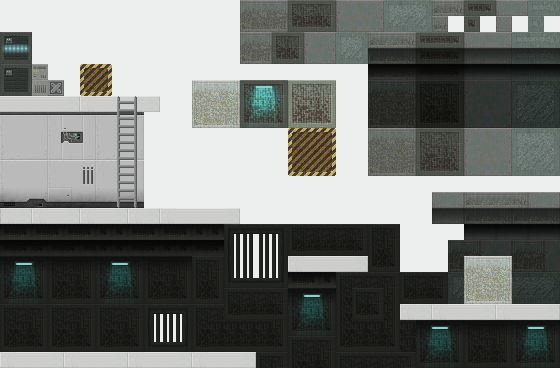
\includegraphics[height=5cm]{images/tileset.jpg}
	\caption{F"ur das Level genutztes Tileset}
	\label{fig:screen_pre}
\end{figure}


Das Level sollte zu Beginn schon einem Turm "ahneln, um an der Spitze den Kampf gegen den Endgegner einzuf"ugen. Ziel beim bauen des Levels war es den Spieler dazu zu bringen alle seine F"ahigkeiten zu nutzen um, m"oglichst unbeschadet, ans Ende des Levels zu kommen und den Endgegner zu besiegen.
Um den Spieler an die Steuerung zu gew"ohnen wird er schon fr"uh mehrere Spr"unge vollf"uhren m"ussen um in den n"achsten Abschnitt zu gelangen. Damit der Spieler nicht st"andig von einer Einer ebene zur n"achsten Springen muss wurden die "Luftstr"ome" eingef"uhrt, die ihn automatisch nach Oben tragen. Um diese darzustellen wurde ein Partikeleffekt genutzt.


\begin{lstlisting}[breaklines=true]
	[...]
	//befindet sich der Spieler innerhalb des Colliders des Luftstrom, so wird ihm in Richtung der
	// y-Achse geschwindigkeit hinzgefuegt
	void OnTriggerStay2D(Collider2D other)
	{
		if(other.tag == "Player")
			other.attachedRigidbody.velocity = new Vector2 (other.attachedRigidbody.velocity.x, other.attachedRigidbody.velocity.y+0.3f);
	}
\end{lstlisting}

Weiterhin wurden T"uren und Aufz"uge genutzt um den Spieler gro"se Abschnitte weiter nach oben Steigen oder ihn ins innere des Turms wechseln zu lassen. Daf"ur wurde ein Script genutzt das aktiviert wird sobald der Spieler innerhalb des Colliders "e" dr"uckt. Dadurch f"arbt sich der Bildschirm schwarz und der Spieler sowie die Kamera wird zur Ausgangst"ur bewegt. Danach klart der Bildschirm wieder auf.

\begin{lstlisting}[breaklines = true]
	[...]
	void OnTriggerStay2D(Collider2D other)
	{
		if (other.tag == "Player" && Input.GetKeyDown ("e") && !isFading) {
			isFading = true;
			fadeToBlack = true;
		}
	}
	
	//Zum aufklaren des Bildschirms
	//Lerpt zwischen der momentanen Farbe der Textur und "Klar" bis der Alphawert der Textur kleiner als 0.1 ist.
	//Danach wird die Farbe auf "Klar" gesetzt.
	void FadeToClear()
	{ 
		fadeTexture.color = Color.Lerp (fadeTexture.color, Color.clear, 1.5f * Time.deltaTime);
		if(fadeTexture.color.a <= 0.1f)
		{
			fadeTexture.color = Color.clear;
			fadeTexture.enabled = false;
			isFading = false;
		}
	}
	
	//Um den Bildschirm schwarz zu faerben
	//Lerpt zwischen der momentanen Farbe der Textur und "Schwarz" bis der Alphawert der Textur groesser als 0.8 ist.
	//Danach wird die Farbe auf "Schwarz" gesetzt.
	void FadeToBlack()
	{
		fadeTexture.enabled = true;
		fadeTexture.color = Color.Lerp (fadeTexture.color, Color.black, 1.5f * Time.deltaTime);
		if (fadeTexture.color.a >= 0.8f) {
			fadeTexture.color = Color.black;
			fadeToBlack = false;
			playerTransform.position = target.position;
			cam.position = new Vector3 (target.position.x, target.position.y, cam.position.z);
		}
	}
\chapter{Men"uf"uhrung}
\chapter{Head-Up-Display \& Tooltips}

\section{Lebens- und Ausdaueranzeige}
\begin{figure}
	\centering
	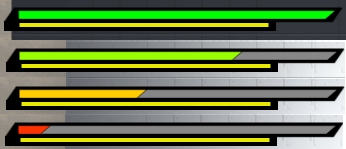
\includegraphics[height=5cm]{images/Lebensleiste.png}
	\caption{Lebensanzeige}
	\label{fig:Lebensanzeige-HUD}
\end{figure}

F"ur das HUD wurde eine Anzeige erstellt, die gleichzeitig auch die Ausdauernd anzeigt. \newline
\begin{lstlisting}[breaklines=true]
//Transform der Lebensleiste
RectTransform healthTransform;
//y-Position der Leiste
float cachedY;
float maxXPos;
float minXPos;
//aktuelle Lebenspunkte
float currentHealth;
float maxHealth;
float newXPos;
AttributeComponent attComp;
Image visualHealth;
\end{lstlisting}
\newpage
An der Stelle an der die Leiste platziert wurde, wurde eine Maske gesetzt. Die Lebenspunkte des Spielers wurden auf die x-Position des Leiste gemappt.\newline

\begin{lstlisting}[breaklines=true]
//Methode zum mappen der Position und Lebenspunkte
private float MapValues(float x, float inMin, float inMax, float outMin, float outMax)
{
	return (x - inMin) * (outMax - outMin) / (inMax - inMin) + outMin;
}

void Update () {
if (currentHealth != attComp.getHealth())
	{
		currentHealth = attComp.getHealth();
		newXPos = MapValues(currentHealth, 0, maxHealth, minXPos, maxXPos);
		healthTransform.localPosition = new Vector3(newXPos, cachedY);
	}
}
\end{lstlisting}
Umso mehr Lebenspunkte der Spieler verliert umso weiter wird die Leiste nach links geschoben. Dank der Maske wird der Teil der Leiste, der "uber sie hinausragt, nicht weiter angezeigt. \newline
\newline Auch wird die Farbe der Leiste zwischen Gr"un und Rot interpoliert, wie in Abbildung 12.1 zu sehen ist.

\begin{lstlisting}[breaklines=true]
if(currentHealth > maxHealth/2)
	{
		visualHealth.color = new Color32((byte)MapValues(currentHealth, maxHealth / 2, maxHealth, 255, 0), 255, 0, 255);
	}

else
	{
		visualHealth.color = new Color32(255, (byte)MapValues(currentHealth, 0, maxHealth / 2, 0, 255), 0, 255);
	}

\end{lstlisting}

F"ur die Ausdaueranzeige wurde ein eigenes Skript geschrieben, welches auf der selben Fuktionsweise basiert, wie die Lebensanzeige, mit dem Unterschied, dass diese sich "uber Zeit von alleine auff"ullt. 
\newpage
\section{Munitionsanzeige}
Auf Tastendruck l"asst sich die Munitionsart des Spielers wechseln. Um dies grafisch zu verdeutlichen wurde am linken unteren Rand ein Panel erstellt, das die Standardmunition beziehungsweise Plasmamunition anzeigt. 
\begin{figure}
	\centering
	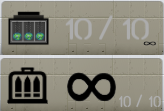
\includegraphics[height=5cm]{images/Munitionsanzeige.png}
	\caption{Munitionsanzeige}
	\label{fig:Munitionsanzeige-HUD}
\end{figure}

\section{Skill-Icons}
Um Abklingzeiten einzuf"uhren und dem Spieler einen Indikator daf"ur zu geben, wie lange er warten muss, bis sich die gew"unschte F"ahigkeit wieder einsetzen zu k"onnen, wurden neben der Munitionsanzeige Icons platziert, die stellvertretend f"ur F"ahigkeiten stehen. Sobald eine F"ahigkeit durch Tastendruck eingesetzt wird, wird das Symbol ausgegraut und die Sekunden bis Freischaltung der F"ahigkeit angezeigt. 
\begin{figure}
	\centering
	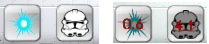
\includegraphics[height=2cm]{images/Skillicons.png}
	\caption{Skill-Icons}
	\label{fig:Skill-Icons-HUD}
\end{figure}
\chapter{Zielsetzung}
\chapter{Abschlussanalyse}
%\input{chapters/TeilnehmerInterviews}
% ...
%--------------------------------------------------------------------------
\backmatter                        		% Anhang
%-------------------------------------------------------------------------
\bibliographystyle{geralpha}			% Literaturverzeichnis
%\bibliography{literatur}     			% BibTeX-File literatur.bib
%--------------------------------------------------------------------------
\printindex 							% Index (optional)
%--------------------------------------------------------------------------
%\begin{appendix}						% Anh�nge sind i.d.R. optional
%   \chapter{Glossar}
			% Glossar   
%\end{appendix}

\end{document}
